\section{Autoionization Processes of Ionized Species}
Vacancies in the core or inner-valence region of atoms and molecules
can decay via photon emission, in case of molecules via coupling to
the nuclear motion or via several autoionization processes. All these
processes compete and hence the fastest are observed. In the auotionization
processes
the vacancy is filled with an electron from an outer shell and the excess
energy is simultaneously transferred to another electron, which consequently
is emitted. Hence the final state is characterized by a doubly ionized state
and an electron in the continuum. These processes can
occur when two criteria are fulfilled, the energy and the coupling criterion.
The energy criterion is fulfilled, when the doubly ionized system in the
final state is of lower energy than the singly ionized initial state.

The different auotionization processes can be classified by the initial
vacancy, where the
vacancy filling electron originates and where the secondary electron is
emitted from.

\subsection{Auger Process}
The Auger process, independently discovered by xyz Auger and Lise Meitner
\cite{}, is the longest known of the presented autoionization processes. Here
the initial ionization mostly resides in the core region of an atom. The vacancy
is then filled by another, energetically higher electron of the same atom, the
energy is simultaneously transferred to yet another electron of the same atom and
emitted as shown in figure \ref{figure:auger_process}.

\begin{figure}[h]
 \centering
 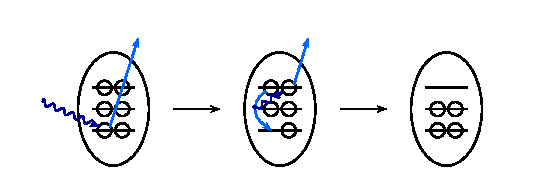
\includegraphics{pics/auger-pspic.eps}
 \caption{}
 \label{figure:auger_process}
\end{figure}


Since both the vacancy filling electron and the emitted electron reside
on the same atom as the initial vacancy, neither energy nor electrons need
to be transferred through space, this process is ultrafast with lifetimes
in the atto- to femtosecond region.

In order to fulfill the energy criterion, the initial ionization has to
be of quite high energy, which is why the process is rarely observed after
ionization from the inner-valence region and therefore the possibility to
observe other autoionization processes.

\subsection{Interatomic Coulombic Decay (ICD)}
The Interatomic/ Intermolecular Coulombic Decay (ICD) was predicted
theoretically 1997 by L. S. Cederbaum \cite{Cederbaum97}
and later verified experimentally by Marburger et al. \cite{Marbuger03}.

Here the initial vacancy is filled by an electron of the same atom and simultaneously,
in contrast to the Auger process, the atom interacts with the surroundings by
transferring the excess energy to another atom, which finally gets ionized. The
positive charges on different atomic sites repell each other and therefore undergo
Coulomb explosion as shown in figure \ref{figure:icd_process}.

\begin{figure}[h]
 \centering
 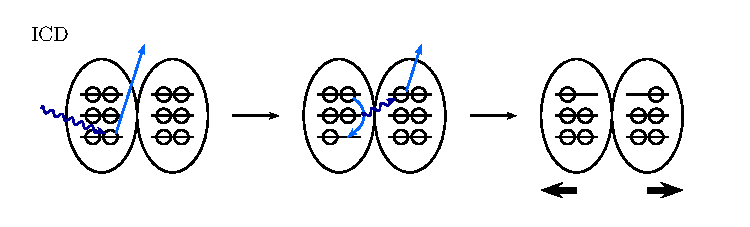
\includegraphics{pics/icd-pspic.eps}
 \caption{}
 \label{figure:icd_process}
\end{figure}

For the following sections we introduce a new nomenclature. The combinations
of all involved atoms and molecules is referred to as the (total) system, whereas
each of them is named a unit. One or a conglomerat of these units, within
the electron fills the vacancy is called a subsystem ($S_1$) as well as the units
forming the 
subsystem emitting the seconday electron $S_2$.

Due to the energy transfer via a virtual photon between to subsystems
the ICD has a lifetime of femto- to pico-seconds.
The initial vacancy of observed ICD processes are normally in the inner-valence,
but are not limited to these cases. Nevertheless, one might rarely observe
an ICD after core ionization, because the Auger process would then be energetically
allowed and outrule the slower ICD.



\subsection{Electron Transfer Mediated Decay Processes}
In the \ac{ETMD} processes the vacancy is filled by an electron from another
atom or molecule. Depending on where the excess energy is transferred to and
hence how many units are involved in the process, the processes are either called
ETMD2 or ETMD3 as shown in figure \ref{figure_etmd_processes}.

\begin{figure}[h]
 \centering
 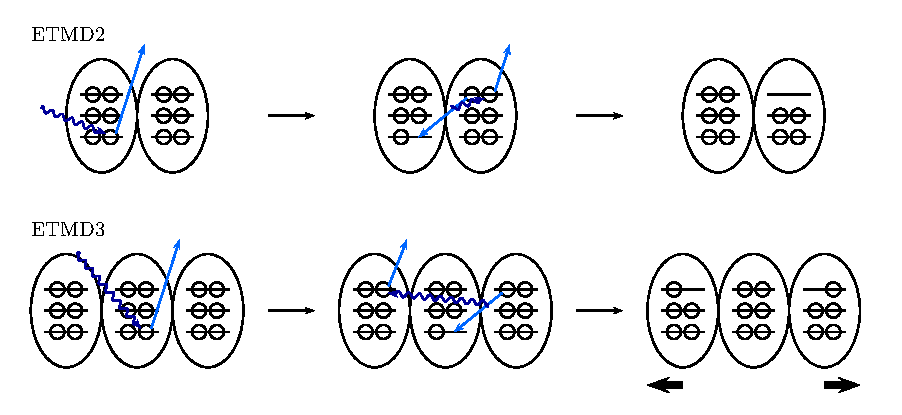
\includegraphics{pics/etmd-pspic.eps}
 \caption{}
 \label{figure:etmd_processes}
\end{figure}

In the ETMD2 the excess energy is transferred to and ionizing an electron
from the vacancy filling unit while in the ETMD3 the excess energy is transferred
to a third unit, which in the nomenclature of the ICD would be subsystem $S_2$.

The decay rate of the process is mostly governed by the electron transfer rate, which
depends on the overlap between the electron clouds of the two units and hence
decreases exponentially with the internuclear/ intermolecular distance. Therefore
the decay rate of the process is normally about two to three orders of magnitude slower
than a competing ICD process and can hence only be observed in cases where either
the ICD is energetically forbidden or, in case of the ETMD3, at interfaces
where the number of potential
triples of atoms is higher and therefore increases the probability for an ETMD3 process
\cite{Fasshauer13}.

The exchange ICD process' decay rate is also governed by the electron transfer
even though it is not evident from its nomenclature. As shown in
figure \ref{figure:exICD_process} the innervalent vacancy is filled by an electron
from the second unit and the excess energy is then transferred back to the first,
initially ionized unit. The two positively charged units then undergo Coulomb
explosion.

\begin{figure}[h]
 \centering
 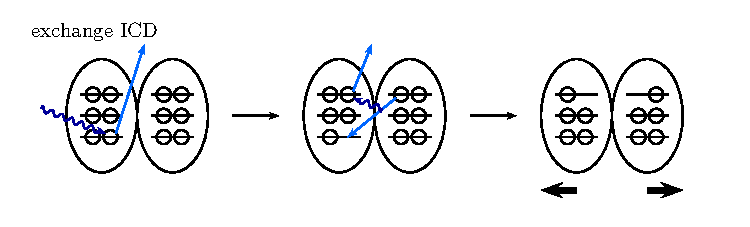
\includegraphics{pics/exicd-pspic.eps}
 \caption{}
 \label{figure:exICD_process}
\end{figure}

Because the final state of the exchange ICD is the same as in the ICD the energy
criterion is the same as for the ICD and the final products are the same. Only
the decay rate is in the range of an ETMD process and hence the process is much
slower than an ICD process. Therefore it is not possible to experimentally
observe and identify this process independently.


\subsection{Resonant ICD (RICD)}
Starting not from an ionized but from an electronically excited state, further
autoionization processes can be observed
as shown in fiure \ref{figure:ricd_processes}.
These electronic decay processes have been known for
the Auger process and been called resonant Auger effect. Analogously ICD like
processes can be initiated by an excitation, which also have been observed
experimentally.

\begin{figure}[h]
 \centering
 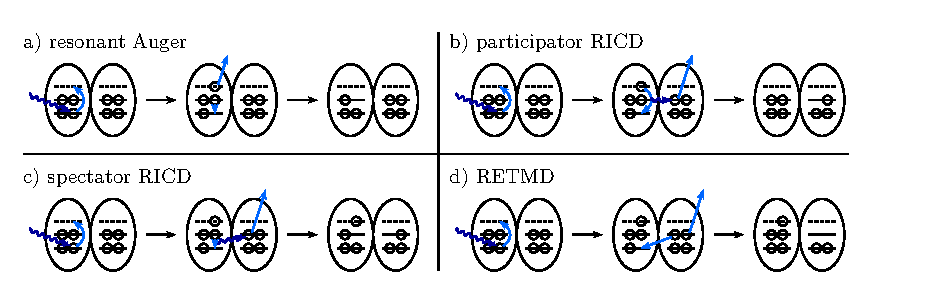
\includegraphics{pics/ricd-pspic.eps}
 \caption{}
 \label{figure:ricd_processes}
\end{figure}

Depending on which role the excited
electron plays in the reaction, the process is either called participator \ac{RICD}
or spectator \ac{RICD}.
In a participator \ac{RICD} the excited electron fills the created vacancy itself.
Simultaneously the excess energy is transferred to a neighbouring unit, which
subsequently gets ioinzed (see figure \ref{figure:ricd_processes} panel b).
The final state is characterized
by the initially excited unit to be in its ground state and the neighbouring atom
being ionized.
In a spectator \ac{RICD} (see figure \ref{figure:ricd_processes} panel c)
the vacancy is filled by another, non-excited electron
of the same unit. The excess energy is simultaneously transferred to a neighbouring
unit, which is then ionized. Throughout the process the excited electron stays
in its virtual orbital.

Recently the special case of a participator \ac{RICD} where the excited
electron stems not from the inner valence but from the outer valence
has been described and has been named \ac{ETI} \cite{Kopelke11}.

As in the case of an ionized initial state also the corresponding ETMD processes
called RETMD (see figure \ref{figure:ricd_processes} panel d) are possible.




\subsection{Interatomic Coulombic Electron Capture (ICEC)}
